\documentclass[aspectratio=169]{beamer}

\usepackage[utf8]{inputenc}
\usetheme{Singapore}
\usepackage{xcolor}
% Colour switches formerly provided by PSTricks, which this deck no longer loads.
\providecommand{\red}{\color{red}}
\providecommand{\blue}{\color{blue}}
\setbeamertemplate{footline}[frame number]

\usepackage{amsmath,amssymb,amsthm}
\usepackage{tikz}
\usetikzlibrary{arrows.meta,decorations.pathreplacing}

\usepackage{times}

\setbeamercovered{dynamic}

\def\RR{\mathbb{R}}

\author[Fabian Bastin]{\texorpdfstring{Fabian Bastin \\ \url{fabian.bastin@umontreal.ca} \\ Université de Montréal -- CIRRELT -- IVADO}{Fabian Bastin}}
\date{}
\title[Linear programming]{Linear programming\\Background material}

\begin{document}

\frame{\titlepage}

\begin{frame}
\frametitle{Linear program}

Linear program, standard form:
\begin{align*}
\min_x\ & c^Tx \\
\mbox{s.t. } & Ax = b,\\
& x \geq 0,
\end{align*}
with $x, c \in \RR^n$, $b \in \RR^m$, $A \in \RR^{m \times n}$.

\mbox{}

Assumptions: rank($A$) = $m$, $m \leq n$.

We write $A_j \in \RR^m$ for the $j$-th {\red column} of $A$, so that the constraints read $\sum_{j=1}^n x_j A_j = b$: a linear program asks for a {\red non-negative} combination of the columns of $A$ that reproduces $b$, at minimum cost.

\mbox{}

Its feasible set is a {\red polyhedron}: a finite intersection of {\red half-spaces} $\lbrace x \mid a^Tx \leq \beta \rbrace$, bounded by the {\red hyperplanes} $\lbrace x \mid a^Tx = \beta \rbrace$.

\end{frame}

\begin{frame}
\frametitle{Standard form}

Any linear program can be transformed to the standard form.
Consider for instance the program
\[
\min_x c^Tx \mbox{ s.t. } Ax \geq b.
\]
Note that there is no sign constraint on $x$.

\mbox{}

We first add a vector $z$ of surplus variables:
\begin{align*}
\min_{x,z}\ & c^Tx \\
\mbox{s.t. } & Ax - z = b,\\
& z \geq 0.
\end{align*}
We next decompose $x$ as the difference of two non-negative variables: $x = x^+-x^-$, where $x^+ = \max \lbrace x,
0 \rbrace \geq 0$, and $x^- = \max \lbrace -x, 0 \rbrace \geq 0$.
\end{frame}

\begin{frame}
\frametitle{Standard form (cont'd)}

The problem becomes
\begin{align*}
\min_{x^+, x^-, z}\ &
\begin{pmatrix}
c^T & -c^T & 0^T
\end{pmatrix}
\begin{pmatrix}
x^+ \\ x^- \\ z
\end{pmatrix}, \\
\mbox{ s.t. } &
\begin{pmatrix}
A & -A & -I
\end{pmatrix}
\begin{pmatrix}
x^+ \\ x^- \\ z
\end{pmatrix} = b,
\begin{pmatrix}
x^+ \\ x^- \\ z
\end{pmatrix} \geq 0.
\end{align*}

The inequality constraints of the form $x \leq u$ or $Ax \leq b$ can be handled by adding slack variables:
\begin{align*}
x \leq u \Leftrightarrow x+w = u,\ w \geq 0, \\
Ax \leq b \Leftrightarrow Ax + y = b,\ y \geq 0.
\end{align*}

\end{frame}

\begin{frame}
\frametitle{Basic solutions}

Without loss of generality, suppose the first $m$ columns of $A$ are independent, and partition $A$ and $x$ accordingly,
\[
A = \begin{pmatrix} B & D \end{pmatrix}, \qquad x = \begin{pmatrix} x_B \\ x_D \end{pmatrix},
\qquad Bx_B + Dx_D = b,
\]
where the {\red basis matrix} $B \in \RR^{m \times m}$ is invertible.

\begin{itemize}
	\item
	{\red Basic solution}: the solution obtained by setting the $n-m$ {\red non-basic} variables to zero, $x_D = 0$, which leaves $x_B = B^{-1}b$ for the {\red basic} ones.
	\item
	{\red Feasible basic solution}: a basic solution with $x_B \geq 0$; then $x \geq 0$, and $x$ is feasible.
	\item
	{\red Degenerate basic solution}: a basic solution with some components of $x_B$ equal to zero. More than $n-m$ variables then vanish, and the same point may come from several bases.
\end{itemize}

\end{frame}

\begin{frame}
\frametitle{A basis of columns, and the coordinates of $b$}

The $m$ columns of $B$ are independent: they form a {\red vector basis of $\RR^m$}.
Choosing a basis is choosing $m$ columns of $A$, and the basic variables are nothing but the {\red coordinates of $b$ in that basis},
\[
b = \sum_{j \in \mathcal{B}} (x_B)_j A_j, \qquad x_B = B^{-1}b,
\]
where $\mathcal{B}$ denotes the set of indices of the chosen columns, the $n-m$ non-basic variables being set to zero.
The basis is {\red feasible} exactly when these coordinates are non-negative, i.e.\ when $b$ lies in the {\red cone} spanned by the chosen columns,
\[
\operatorname{cone}\lbrace v^1, \ldots, v^k \rbrace \overset{\mathrm{def}}{=} \lbrace \lambda_1 v^1 + \cdots + \lambda_k v^k \mid \lambda \geq 0 \rbrace,
\]
and not merely in the subspace they span: the span only asks that $b$ be reachable, the cone asks that it be reachable with {\red non-negative} weights.

\end{frame}

\begin{frame}
\frametitle{Two bases, two sets of coordinates}

\vspace{-1mm}

{\footnotesize $A = \begin{pmatrix} 2 & 1 & -1 & 0 \\ 0 & 2 & 1 & 1\end{pmatrix}$, $b = \begin{pmatrix} 3 \\ 2\end{pmatrix}$: both column pairs below are bases of $\RR^2$, only the first one is feasible.}

\begin{center}
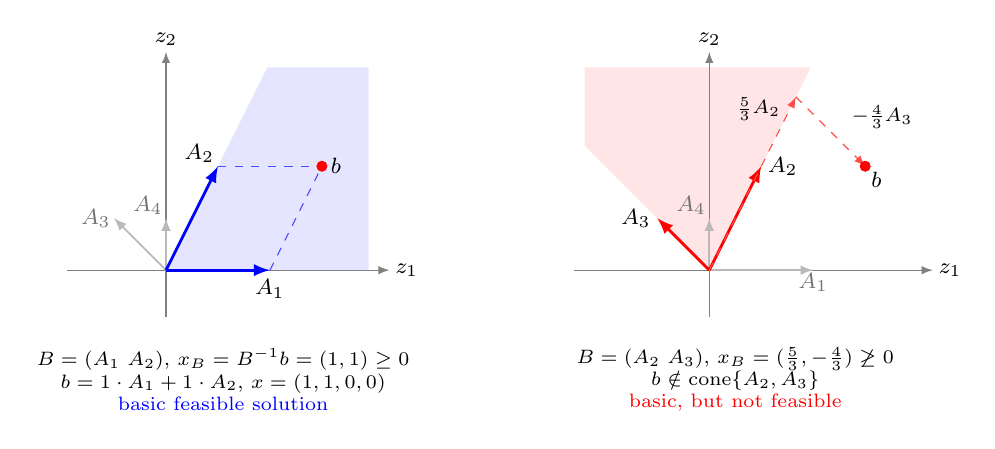
\begin{tikzpicture}[x=0.66cm,y=0.66cm,>=latex,font=\footnotesize]
  % ---------------- panel A: feasible basis (A1, A2)
  \fill[blue!10] (0,0) -- (3.9,0) -- (3.9,3.9) -- (1.95,3.9) -- cycle;
  \draw[->,gray] (-1.9,0) -- (4.3,0) node[right,black,inner sep=2pt]{$z_1$};
  \draw[->,gray] (0,-0.9) -- (0,4.2) node[above,black,inner sep=2pt]{$z_2$};
  \draw[->,gray!55,line width=0.6pt] (0,0) -- (-1,1) node[left,black!55,inner sep=1pt]{$A_3$};
  \draw[->,gray!55,line width=0.6pt] (0,0) -- (0,1) node[above left,black!55,inner sep=1pt]{$A_4$};
  \draw[->,blue,line width=1pt] (0,0) -- (2,0) node[below,black,inner sep=3pt]{$A_1$};
  \draw[->,blue,line width=1pt] (0,0) -- (1,2) node[above left,black,inner sep=1pt]{$A_2$};
  \draw[dashed,blue!70] (2,0) -- (3,2);
  \draw[dashed,blue!70] (1,2) -- (3,2);
  \fill[red] (3,2) circle (2pt) node[right,black,inner sep=3pt]{$b$};
  \node[align=center,font=\scriptsize] at (1.1,-2.1)
     {$B=(A_1\ A_2)$, $x_B = B^{-1}b = (1,1) \geq 0$\\
      $b = 1 \cdot A_1 + 1 \cdot A_2$, $x = (1,1,0,0)$\\
      {\blue basic feasible solution}};
  % ---------------- panel B: infeasible basis (A2, A3)
  \begin{scope}[xshift=6.9cm]
    \fill[red!10] (0,0) -- (1.95,3.9) -- (-2.4,3.9) -- (-2.4,2.4) -- cycle;
    \draw[->,gray] (-2.6,0) -- (4.3,0) node[right,black,inner sep=2pt]{$z_1$};
    \draw[->,gray] (0,-0.9) -- (0,4.2) node[above,black,inner sep=2pt]{$z_2$};
    \draw[->,gray!55,line width=0.6pt] (0,0) -- (2,0) node[below,black!55,inner sep=1pt]{$A_1$};
    \draw[->,gray!55,line width=0.6pt] (0,0) -- (0,1) node[above left,black!55,inner sep=1pt]{$A_4$};
    \draw[->,red,line width=1pt] (0,0) -- (1,2) node[right,black,inner sep=2pt]{$A_2$};
    \draw[->,red,line width=1pt] (0,0) -- (-1,1) node[left,black,inner sep=2pt]{$A_3$};
    \draw[dashed,red!70,->] (0,0) -- (1.667,3.333);
    \node[black,font=\scriptsize,left] at (1.55,3.1) {$\tfrac{5}{3}A_2$};
    \draw[dashed,red!70,->] (1.667,3.333) -- (3,2);
    \node[black,font=\scriptsize,right] at (2.55,2.95) {$-\tfrac{4}{3}A_3$};
    \fill[red] (3,2) circle (2pt) node[below right,black,inner sep=2pt]{$b$};
    \node[align=center,font=\scriptsize] at (0.5,-2.1)
      {$B=(A_2\ A_3)$, $x_B = (\tfrac{5}{3},-\tfrac{4}{3}) \not\geq 0$\\
       $b \notin \operatorname{cone}\lbrace A_2,A_3 \rbrace$\\
       {\red basic, but not feasible}};
  \end{scope}
\end{tikzpicture}
\end{center}

\end{frame}

\begin{frame}
	\frametitle{Fundamental theorem of linear programming}

Consider an LP in standard form, with $A \in \RR^{m \times n}$, and rank($A$) = $m$.
	\begin{itemize}
		\item
		If there exists a feasible solution, then there exists a feasible basic solution.
		\item
		If there exists a feasible optimal solution, then there exists a feasible optimal basic solution.
	\end{itemize}

\mbox{}

The search for an optimum can therefore be restricted to the {\red finitely many} choices of $m$ columns out of $n$: this is what the simplex method exploits, moving from one basis to an adjacent one.

\end{frame}

\begin{frame}
\frametitle{Bases and vertices}

\vspace{-1mm}

{\footnotesize $\lbrace x \in \RR^2_+ \mid x_1 \leq 3,\ x_2 \leq 2,\ x_1 + x_2 \leq 4 \rbrace$, put in standard form with the slacks $w_1, w_2, w_3$: $m = 3$, $n = 5$. Each vertex is labelled by its basis.}

\begin{center}
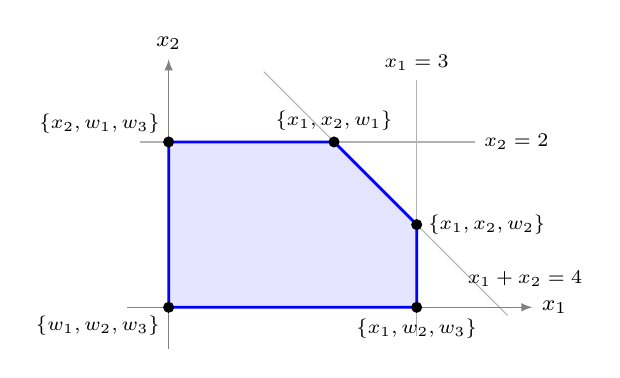
\begin{tikzpicture}[x=1.05cm,y=1.05cm,>=latex,font=\footnotesize]
  \fill[blue!10] (0,0) -- (3,0) -- (3,1) -- (2,2) -- (0,2) -- cycle;
  \draw[gray!60] (3,-0.35) -- (3,2.75) node[above,black,font=\scriptsize]{$x_1=3$};
  \draw[gray!60] (-0.35,2) -- (3.7,2);
  \node[black,font=\scriptsize,right] at (3.7,2) {$x_2=2$};
  \draw[gray!60] (1.15,2.85) -- (4.1,-0.1);
  \node[black,font=\scriptsize,right] at (3.5,0.35) {$x_1+x_2=4$};
  \draw[->,gray] (-0.5,0) -- (4.4,0) node[right,black]{$x_1$};
  \draw[->,gray] (0,-0.5) -- (0,3.0) node[above,black]{$x_2$};
  \draw[blue,line width=1pt] (0,0) -- (3,0) -- (3,1) -- (2,2) -- (0,2) -- cycle;
  \fill (0,0) circle (2pt);  \node[font=\scriptsize,below left,inner sep=3pt] at (0,0) {$\lbrace w_1,w_2,w_3 \rbrace$};
  \fill (3,0) circle (2pt);  \node[font=\scriptsize,below,inner sep=4pt] at (3,0) {$\lbrace x_1,w_2,w_3 \rbrace$};
  \fill (3,1) circle (2pt);  \node[font=\scriptsize,right,inner sep=4pt] at (3,1) {$\lbrace x_1,x_2,w_2 \rbrace$};
  \fill (2,2) circle (2pt);  \node[font=\scriptsize,above,inner sep=4pt] at (2,2) {$\lbrace x_1,x_2,w_1 \rbrace$};
  \fill (0,2) circle (2pt);  \node[font=\scriptsize,above left,inner sep=3pt] at (0,2) {$\lbrace x_2,w_1,w_3 \rbrace$};
\end{tikzpicture}
\end{center}

\vspace{-2mm}

{\footnotesize The $n-m = 2$ non-basic variables are exactly those vanishing at the vertex: the five vertices are the five feasible bases among the $\binom{5}{3} = 10$ column triples (two of which are singular, three basic but infeasible).}

\end{frame}

\begin{frame}
\frametitle{Convex sets and convex functions}

\begin{itemize}
	\item
	A {\red convex combination} of $x^1, \ldots, x^k$ is $\sum_{i=1}^k \lambda_i x^i$ with $\lambda \geq 0$ and $\sum_{i=1}^k \lambda_i = 1$.
	Dropping the normalisation $\sum_i \lambda_i = 1$ gives back the non-negative combinations that generate a cone.
	\item
	A set $C$ is {\red convex} if it contains the convex combinations of its points, equivalently the segment $[x,y]$ for all $x, y \in C$.
	A half-space is convex, and so is any intersection of half-spaces: {\red a polyhedron is convex}.
	\item
	A function $f$ is {\red convex} if
	\[
	f(\lambda x + (1-\lambda)y) \leq \lambda f(x) + (1-\lambda) f(y), \quad x, y \in \RR^n,\ \lambda \in [0,1].
	\]
	A maximum of linear functions is convex --- which is what will make the value function of a linear program convex.
\end{itemize}

\end{frame}

\begin{frame}
\frametitle{Extreme points and extreme rays}

Let $P = \lbrace x \,|\, Ax = b,\ x \geq 0 \rbrace$ be non-empty.
\begin{itemize}
	\item
	$x \in P$ is an {\red extreme point} (or vertex) of $P$ if it is not a strict convex combination of two points of $P$:
	\[
	x = \lambda y + (1-\lambda)z,\ y, z \in P,\ \lambda \in (0,1) \quad \Longrightarrow \quad y = z = x.
	\]
	($P$ being convex, testing $\lambda = \tfrac12$ is already enough.)
	\item
	The {\red recession cone} of $P$ is $C = \lbrace d \,|\, Ad = 0,\ d \geq 0 \rbrace$: the directions along which $P$ is unbounded, $x + \alpha d \in P$ for every $x \in P$ and $\alpha \geq 0$.
	For $d \in C \setminus \lbrace 0 \rbrace$, the half-line $\lbrace \alpha d \,|\, \alpha \geq 0 \rbrace$ is a {\red ray} of $P$.
	\item
	That ray is an {\red extreme ray} if every decomposition of $d$ inside $C$ stays on the ray:
	\[
	d = d^1 + d^2,\ d^1, d^2 \in C \quad \Longrightarrow \quad d^1, d^2 \text{ are non-negative multiples of } d.
	\]
	Being half-lines, rays are counted {\red up to a positive factor}.
\end{itemize}

\end{frame}

\begin{frame}
\frametitle{Extreme points and extreme rays (cont'd)}

\begin{itemize}
	\item
	The extreme points of $P$ are exactly its feasible basic solutions. Distinct extreme points have distinct bases, hence there are {\red finitely many}: at most $\binom{n}{m}$. That bound is crude --- most column subsets are singular or infeasible --- but the simplex $\lbrace x \geq 0 \mid \sum_j x_j = 1 \rbrace$ attains it, with $n$ vertices.
	\item
	The rays obey the same mechanism: writing $S = \lbrace j \,|\, d_j > 0 \rbrace$, the ray of $d \in C$ is extreme if and only if the columns $A_j$, $j \in S$, have rank $|S|-1$ --- they carry exactly one dependency, and $d$ is it.
	The extreme rays are therefore {\red finite} in number too.
	\item
	More generally, the recession cone of $\lbrace \pi \,|\, A^T\pi \leq c \rbrace$ is $\lbrace \sigma \,|\, A^T\sigma \leq 0 \rbrace$: this is the form met in the dual problems below.
	\item
	{\red Resolution theorem}: every $x \in P$ is the sum of a convex combination of the extreme points and of a non-negative combination of the extreme rays.
\end{itemize}

Consequently a linear program over $P$ attains its optimum at an extreme point, or is unbounded along an extreme ray $r$ with $c^Tr < 0$.

\end{frame}

\begin{frame}
\frametitle{Extreme points and extreme rays, graphically}

\begin{center}
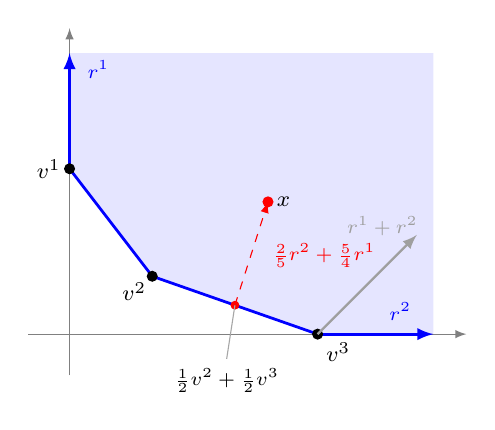
\begin{tikzpicture}[x=1.05cm,y=1.05cm,>=latex,font=\footnotesize]
  \fill[blue!10] (0,2) -- (1,0.7) -- (3,0) -- (4.4,0) -- (4.4,3.4) -- (0,3.4) -- cycle;
  \draw[->,gray] (-0.5,0) -- (4.8,0);
  \draw[->,gray] (0,-0.5) -- (0,3.7);
  \draw[blue,line width=1pt] (0,2) -- (1,0.7) -- (3,0);
  \draw[->,blue,line width=1pt] (0,2) -- (0,3.4);
  \draw[->,blue,line width=1pt] (3,0) -- (4.4,0);
  \fill (0,2) circle (2pt) node[left,black,inner sep=3pt]{$v^1$};
  \fill (1,0.7) circle (2pt) node[below left,black,inner sep=2pt]{$v^2$};
  \fill (3,0) circle (2pt) node[below right,black,inner sep=3pt]{$v^3$};
  \node[blue,font=\scriptsize,right] at (0.1,3.2) {$r^1$};
  \node[blue,font=\scriptsize,above] at (4.0,0.05) {$r^2$};
  \draw[->,gray!75,line width=0.8pt] (3,0) -- (4.2,1.2);
  \node[gray!75,font=\scriptsize,above left,inner sep=1pt] at (4.25,1.15) {$r^1+r^2$};
  % decomposition of a point
  \fill[red] (2,0.35) circle (1.6pt);
  \draw[gray!70,line width=0.4pt] (2,0.35) -- (1.9,-0.3);
  \node[black,font=\scriptsize,below] at (1.9,-0.3) {$\tfrac12 v^2 + \tfrac12 v^3$};
  \draw[->,red,dashed] (2,0.35) -- (2.4,1.6);
  \fill[red] (2.4,1.6) circle (2pt) node[right,black,inner sep=3pt]{$x$};
  \node[red,font=\scriptsize,right] at (2.34,0.95) {$\tfrac{2}{5}r^2 + \tfrac{5}{4}r^1$};
\end{tikzpicture}
\end{center}

\vspace{-2mm}

{\footnotesize Three extreme points, two extreme rays; $r^1+r^2$ is a recession direction of $P$, but not an extreme one, since it splits along two rays of different directions. Every $x \in P$ is a convex combination of the $v^i$ plus a non-negative combination of the $r^j$. The optimum of $c^Tx$ is attained at some $v^i$, unless $c^Tr^j < 0$ for some $j$.}

\end{frame}

\begin{frame}
\frametitle{When does a polyhedron have extreme points?}

$P$ contains a {\red line} if $x + \alpha d \in P$ for some $x \in P$, some $d \neq 0$ and \emph{every} $\alpha \in \RR$ --- equivalently, if $d$ and $-d$ both lie in the recession cone.

\vspace{1.5mm}

A non-empty polyhedron has an extreme point {\red if and only if} it contains no line. It is then said to be {\red pointed}.

\vspace{-1mm}

\begin{center}
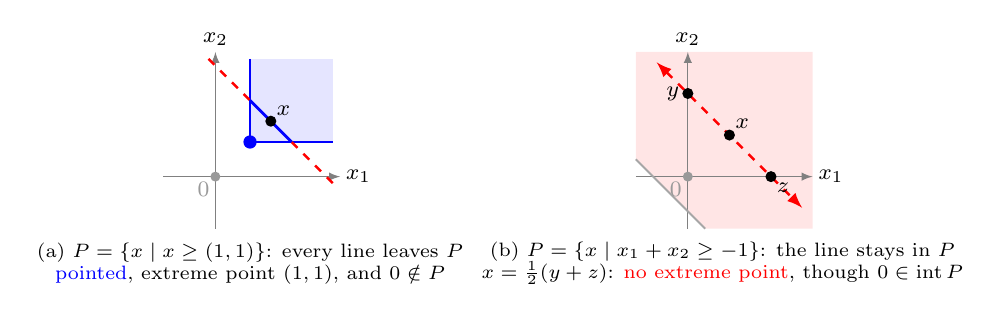
\begin{tikzpicture}[x=0.44cm,y=0.44cm,>=latex,font=\footnotesize]
  % ---------------- (a) a translated orthant: pointed, and 0 is outside it
  \fill[blue!10] (1,1) rectangle (3.4,3.4);
  \draw[->,gray] (-1.5,0) -- (3.6,0) node[right,black,inner sep=2pt]{$x_1$};
  \draw[->,gray] (0,-1.5) -- (0,3.6) node[above,black,inner sep=2pt]{$x_2$};
  \draw[blue,line width=0.8pt] (1,3.4) -- (1,1) -- (3.4,1);
  \draw[red,dashed,line width=0.9pt] (-0.2,3.4) -- (1,2.2);
  \draw[red,dashed,line width=0.9pt] (2.2,1) -- (3.4,-0.2);
  \draw[blue,line width=1pt] (1,2.2) -- (2.2,1);
  \fill (1.6,1.6) circle (2pt) node[above right,black,inner sep=2pt]{$x$};
  \fill[blue] (1,1) circle (2.4pt);
  \fill[gray!80] (0,0) circle (1.8pt) node[below left,gray!80,inner sep=2pt]{$0$};
  \node[align=center,font=\scriptsize] at (1.0,-2.5)
    {(a) $P = \lbrace x \mid x \geq (1,1) \rbrace$: every line leaves $P$\\{\blue pointed}, extreme point $(1,1)$, and $0 \notin P$};
  % ---------------- (b) a half-space: no extreme point, and 0 is interior
  \begin{scope}[xshift=6.0cm]
    \fill[red!10] (-1.5,0.5) -- (0.5,-1.5) -- (3.6,-1.5) -- (3.6,3.6) -- (-1.5,3.6) -- cycle;
    \draw[->,gray] (-1.5,0) -- (3.6,0) node[right,black,inner sep=2pt]{$x_1$};
    \draw[->,gray] (0,-1.5) -- (0,3.6) node[above,black,inner sep=2pt]{$x_2$};
    \draw[gray!70,line width=0.7pt] (-1.5,0.5) -- (0.5,-1.5);
    \draw[red,dashed,line width=0.9pt,<->] (-0.9,3.3) -- (3.3,-0.9);
    \fill (0,2.4) circle (2pt) node[left,black,inner sep=3pt]{$y$};
    \fill (2.4,0) circle (2pt) node[below right,black,inner sep=2pt]{$z$};
    \fill (1.2,1.2) circle (2pt) node[above right,black,inner sep=2pt]{$x$};
    \fill[gray!80] (0,0) circle (1.8pt) node[below left,gray!80,inner sep=2pt]{$0$};
    \node[align=center,font=\scriptsize] at (1.0,-2.5)
      {(b) $P = \lbrace x \mid x_1+x_2 \geq -1 \rbrace$: the line stays in $P$\\$x = \tfrac12(y+z)$: {\red no extreme point}, though $0 \in \operatorname{int} P$};
  \end{scope}
\end{tikzpicture}
\end{center}

{\footnotesize Translation leaves $C$ unchanged, so the origin plays no role. In standard form $C \subseteq \RR^n_+$, and $d, -d \in C$ force $d = 0$: $x \geq 0$ alone makes $P$ pointed. The dual polyhedron is shaped like (b), where rank($A$) $= m$ excludes lines.}

\end{frame}

\begin{frame}
	\frametitle{Duality: symmetric form}

\begin{itemize}
	\item 
{\red Primal} program
\begin{equation}
	\begin{aligned}
	\min_{x \geq 0} \ & c^T x \\
	\mbox{s.t. } & Ax \geq b
	\end{aligned}
\tag{P}\label{eq:primal}
\end{equation}
\item
{\red Dual} program
\begin{equation}
	\begin{aligned}
	\max_{\pi \geq 0} \ & \pi^T b \\
	\mbox{s.t. } & A^T \pi \leq c
	\end{aligned}
\tag{D}\label{eq:dual}
\end{equation}
\item
$A \in \RR^{m \times n}$, $c, x \in \RR^n$, $\pi, b \in \RR^m$: $x$ gathers the {\red primal} variables, $\pi$ the {\red dual} ones.
\item
Dualizing (D) gives (P) back: the dual of the dual is the primal.
\end{itemize}
\end{frame}

\begin{frame}
	\frametitle{Duality: from the standard form}
	
	The program
	\begin{align*}
		\min_x \ & c^T x \\
		\mbox{s.t. } & Ax = b \\
		& x \geq 0
	\end{align*}
	is equivalent to
	\begin{align*}
		\min_x \ & c^T x \\
		\mbox{s.t. } & Ax \geq b \\
		& -Ax \geq -b \\
		& x \geq 0
	\end{align*}
	
\end{frame}

\begin{frame}
	\frametitle{Duality: asymmetric form}
	
The dual problem can then be written as
	\begin{align*}
		\max_{u, v} \ & u^T b - v^T b \\
		\mbox{s.t. } & u^T A - v^T A \leq c^T \\
		& u \geq 0 \\
		& v \geq 0
	\end{align*}
	or, with $\pi = u - v$,
	\begin{align*}
		\max_{\pi} \ & \pi^T b \\
		\mbox{s.t. } & \pi^T A \leq c^T
	\end{align*}
	
Asymmetric form: $\pi \in \RR^m$ is unrestricted in sign.
	
\end{frame}


\begin{frame}
	\frametitle{Primal-dual conversion}
	
	\begin{center}
		\begin{tabular}{|c|c|}
			\hline
			\hline
			{\bf Minimization} & {\bf Maximization} \\
			\hline
			\hline
			Constraints & Variables \\
			\hline
			$\geq$ & $\geq 0$ \\
			$\leq$ & $\leq 0$ \\
			$=$ & unconstrained \\
			\hline
			\hline
			Variables & Constraints \\
			\hline
			$\geq 0$ & $\leq$ \\
			$\leq 0$ & $\geq$ \\
			unconstrained & $=$ \\
			\hline
		\end{tabular}
	\end{center}
	
\end{frame}

\begin{frame}
	\frametitle{Weak duality}
	
	(Asymmetric or symmetric form)
	
	\mbox{}
	
	If $x$ and $\pi$ are feasible for the primal and the dual, respectively, then
	\[
	c^T x \geq \pi^T b
	\]
	
	\begin{proof}
		For any primal feasible $x$ and dual feasible $\pi$, we have
		\[
		\pi^T b \leq \pi^TAx \leq c^Tx,
		\]
		the first inequality because $\pi \geq 0$ and $Ax \geq b$ (an equality in the asymmetric form, where $Ax = b$), the second because $x \geq 0$ and $A^T\pi \leq c$.
	\end{proof}
	
\end{frame}

\begin{frame}
	\frametitle{Corollary}
	
	If $x_0$ and $\pi_0$ are feasible for the primal and the dual, respectively, and if
	\[
	c^T x_0 = \pi_0^T b,
	\]
	then $x_0$ and $\pi_0$ are optimal for their respective problem.
	
	\mbox{}
	
	But we have said nothing about the feasibility of one problem with respect to the other one!
	
\end{frame}

\begin{frame}
	\frametitle{Weak and strong duality, graphically}

\begin{center}
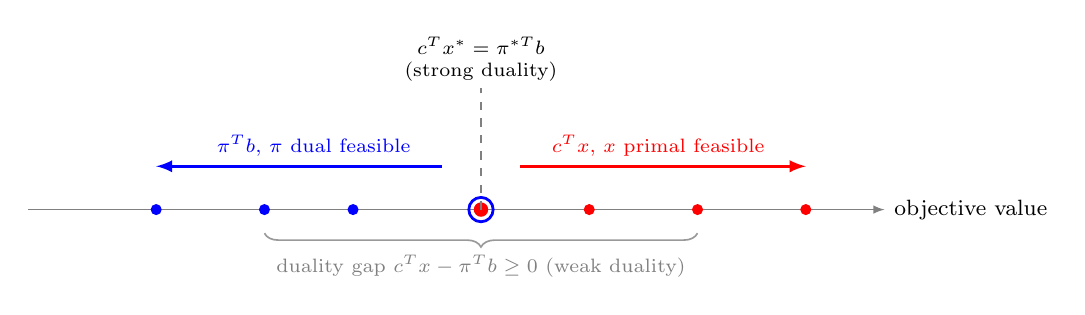
\begin{tikzpicture}[x=1.25cm,y=1cm,>=latex,font=\footnotesize]
  \draw[->,gray] (-0.3,0) -- (8.4,0) node[right,black]{objective value};
  % dual feasible values
  \foreach \p in {1.0,2.1,3.0} \fill[blue] (\p,0) circle (2pt);
  % primal feasible values
  \foreach \p in {5.4,6.5,7.6} \fill[red] (\p,0) circle (2pt);
  % common optimal value: dual mark and primal mark coincide
  \fill[red] (4.3,0) circle (2.6pt);
  \draw[blue,line width=1pt] (4.3,0) circle (4.4pt);
  \draw[blue,line width=1pt,->] (3.9,0.55) -- (1.0,0.55);
  \node[blue,above,font=\scriptsize] at (2.6,0.55) {$\pi^Tb$, $\pi$ dual feasible};
  \draw[red,line width=1pt,->] (4.7,0.55) -- (7.6,0.55);
  \node[red,above,font=\scriptsize] at (6.1,0.55) {$c^Tx$, $x$ primal feasible};
  \draw[decorate,decoration={brace,mirror,amplitude=5pt},gray!80,line width=0.6pt] (2.1,-0.3) -- (6.5,-0.3);
  \node[below,font=\scriptsize,gray] at (4.3,-0.45) {duality gap $c^Tx - \pi^Tb \geq 0$ (weak duality)};
  \draw[dashed,gray] (4.3,0) -- (4.3,1.55);
  \node[above,font=\scriptsize,align=center] at (4.3,1.5) {$c^Tx^* = \pi^{*T}b$\\{\scriptsize (strong duality)}};
\end{tikzpicture}
\end{center}

\vspace{-1mm}

{\footnotesize Every dual feasible value bounds every primal feasible value from below. Strong duality states that the two families actually {\red meet}: the best lower bound is the optimal value. The corollary above is read on the picture: a blue and a red mark that coincide can only sit at the meeting point.}

\end{frame}

\begin{frame}
	\frametitle{Strong duality}
	
	If one of the problems \eqref{eq:primal} or \eqref{eq:dual} has a finite optimal solution, the other problem also has a finite optimal solution, and the corresponding values of the objective functions are equal.
	If one of the problems has an unbounded objective, the other problem has no feasible solution.

\mbox{}

If a program is infeasible, this does not imply that its dual is unbounded: it can be infeasible as well.
In the table below, ``bounded'' means that the program is feasible and has a finite optimal value.

\mbox{}

\begin{center}
	\begin{tabular}{|c||c|c|c|}
		\hline
		Primal / Dual & Bounded & Unbounded & Infeasible \\
		\hline
		\hline
		Bounded & possible & impossible & impossible \\
		\hline
		Unbounded & impossible & impossible & possible \\
		\hline
		Infeasible & impossible & possible & possible \\
		\hline
	\end{tabular}
\end{center}

\end{frame}

\begin{frame}
\frametitle{Polyhedral cones and Farkas' lemma}

{\red Positive hull}: the cone of the previous slides, now generated by {\red all} the columns of $A$ at once,
\[
\text{pos}\,A = \operatorname{cone}\lbrace A_1, \ldots, A_n \rbrace = \lbrace z \,|\, z = Ax,\ x \geq 0 \rbrace.
\]
It is exactly the set of right-hand sides $z$ for which $Ax = z$, $x \geq 0$, admits a solution.

\begin{block}{Farkas' lemma}
Let $A \in \RR^{m \times n}$ and $b \in \RR^m$. Exactly one of the following holds:
\begin{itemize}
	\item
	$\exists\, x \geq 0$ such that $Ax = b$, i.e. $b \in \text{pos}\,A$;
	\item
	$\exists\, u \in \RR^m$ such that $A^Tu \geq 0$ and $b^Tu < 0$.
\end{itemize}
\end{block}

The second vector is a {\red certificate of infeasibility}: it defines a hyperplane separating $b$ from $\text{pos}\,A$.
One may always take $u$ on an extreme ray of $\lbrace u \,|\, A^Tu \geq 0 \rbrace$, so that finitely many certificates suffice.

\end{frame}

\begin{frame}
\frametitle{Farkas' lemma, graphically}

\begin{center}
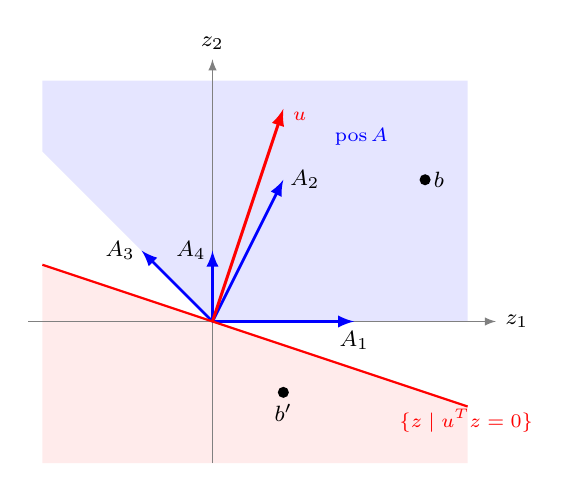
\begin{tikzpicture}[x=0.9cm,y=0.9cm,>=latex,font=\footnotesize]
  \fill[blue!10] (0,0) -- (3.6,0) -- (3.6,3.4) -- (-2.4,3.4) -- (-2.4,2.4) -- cycle;
  \fill[red!8] (-2.4,0.8) -- (3.6,-1.2) -- (3.6,-2.0) -- (-2.4,-2.0) -- cycle;
  \draw[->,gray] (-2.6,0) -- (4.0,0) node[right,black]{$z_1$};
  \draw[->,gray] (0,-2.0) -- (0,3.7) node[above,black]{$z_2$};
  \draw[->,blue,line width=1pt] (0,0) -- (2,0) node[below,black,inner sep=3pt]{$A_1$};
  \draw[->,blue,line width=1pt] (0,0) -- (1,2) node[right,black,inner sep=2pt]{$A_2$};
  \draw[->,blue,line width=1pt] (0,0) -- (-1,1) node[left,black,inner sep=2pt]{$A_3$};
  \draw[->,blue,line width=1pt] (0,0) -- (0,1) node[left,black,inner sep=2pt]{$A_4$};
  \node[blue,font=\scriptsize] at (2.1,2.6) {$\text{pos}\,A$};
  \draw[red,line width=0.8pt] (-2.4,0.8) -- (3.6,-1.2);
  \node[red,font=\scriptsize,below right] at (2.5,-1.1) {$\lbrace z \mid u^Tz = 0 \rbrace$};
  \draw[->,red,line width=1.1pt] (0,0) -- (1,3);
  \node[red,font=\scriptsize,right] at (1.0,2.9) {$u$};
  \fill[black] (3,2) circle (2pt) node[right,inner sep=3pt]{$b$};
  \fill[black] (1,-1) circle (2pt) node[below,inner sep=4pt]{$b'$};
\end{tikzpicture}
\end{center}

\vspace{-2mm}

{\footnotesize Same columns as before: $b = (3,2)$ lies in the blue cone, so $Ax = b$, $x \geq 0$ is solvable. $b' = (1,-1)$ does not, and $u = (1,3)$ certifies it: $A^Tu = (2,7,2,3) \geq 0$ while $u^Tb' = -2 < 0$. The red half-space $\lbrace z \mid u^Tz < 0 \rbrace$ holds $b'$ and misses the cone.}

\end{frame}

\begin{frame}
\frametitle{The polar cone}
\small

The {\red polar} of a cone $C \subseteq \RR^m$ is
\[
C^{\circ} \overset{\mathrm{def}}{=} \lbrace u \mid u^Tz \leq 0 \ \ \forall z \in C \rbrace,
\]
the directions making an obtuse angle with everything in $C$. For $C = \text{pos}\,A$ it is read off $A$:
\[
\lbrace u \mid A^Tu \leq 0 \rbrace
= \lbrace u \mid y^TA^Tu \leq 0\ \forall y \geq 0 \rbrace
= \lbrace u \mid u^T(Ay) \leq 0\ \forall y \geq 0 \rbrace
= (\text{pos}\,A)^{\circ},
\]
the first equality because $A^Tu \leq 0$ componentwise is the same as $y^T(A^Tu) \leq 0$ for all $y \geq 0$.

Farkas' lemma says $b \in \text{pos}\,A$ iff $A^Tu \geq 0 \Rightarrow b^Tu \geq 0$; replacing $u$ by $-u$, legitimate since it holds for every $u$, gives $A^Tu \leq 0 \Rightarrow b^Tu \leq 0$, that is
\[
b \in \text{pos}\,A \iff b^Tu \leq 0 \ \ \text{for every } u \in (\text{pos}\,A)^{\circ}.
\]

{\footnotesize So the polar collects the {\red certificates of infeasibility}: a single $u$ in it with $b^Tu > 0$ proves that $Ax = b$, $x \geq 0$ has no solution. In the recourse problems of the following decks, $\text{pos}\,W$ is the set of right-hand sides the second stage can absorb, and the elements of its polar are exactly what the decomposition methods turn into {\red feasibility cuts}.}

\end{frame}

\begin{frame}
\frametitle{Optimality conditions for a linear program}

Specialising the KKT conditions to a linear program, $x$ is optimal {\red if and only if} there are $\pi \in \RR^m$ and $s \in \RR^n$ with
\begin{align*}
Ax = b,\ x &\geq 0 &&\text{(primal feasibility)},\\
A^T\pi + s = c,\ s &\geq 0 &&\text{(dual feasibility)},\\
x_is_i &= 0,\ i = 1, \ldots, n &&\text{({\red complementary slackness})}.
\end{align*}

\begin{itemize}
	\item
	In LP no constraint qualification is needed, and the conditions are {\red sufficient} as well as necessary --- both are specific to the linear (convex, polyhedral) case.
	\item
	They give strong duality in one line: $c^Tx = (A^T\pi+s)^Tx = \pi^TAx + s^Tx = \pi^Tb$, using $s^Tx = 0$ and $Ax = b$.
	\item
	Complementary slackness is what lets one read off the optimal $y$ from an optimal $\pi$ in the recourse problems of the following decks.
\end{itemize}

The Lagrangian, the general KKT conditions, constraint qualifications and the duality gap are treated in the {\red KKT background notes}.

\end{frame}

\begin{frame}
\frametitle{The value function of a linear program}

Consider the optimal value as a function of the right-hand side,
\[
z(b) \overset{\mathrm{def}}{=} \min_x \lbrace c^Tx \,|\, Ax = b,\ x \geq 0 \rbrace,
\]
with $z(b) = +\infty$ when the program is infeasible: its {\red domain} $\operatorname{dom} z = \lbrace b \,|\, z(b) < +\infty \rbrace$ is exactly $\text{pos}\,A$.

\mbox{}

By duality, $z(b) = \max_{\pi} \lbrace \pi^Tb \,|\, A^T\pi \leq c \rbrace$, where the feasible set {\red does not depend on $b$}.
Assume it non-empty (otherwise $z \equiv -\infty$ on $\text{pos}\,A$); rank($A$) $= m$ makes it pointed, so it has extreme points $\pi^1, \ldots, \pi^r$ and, for $b \in \operatorname{dom} z$,
\[
z(b) = \max_{i = 1,\ldots,r} (\pi^i)^Tb.
\]

\end{frame}

\begin{frame}
\frametitle{Subgradients and supporting hyperplanes}

A vector $g$ is a {\red subgradient} of a convex function $f$ at $b$ if it supports $f$ from below everywhere,
\[
f(b') \geq f(b) + g^T(b'-b) \quad \text{for all } b',
\]
and the set of them is the {\red subdifferential} $\partial f(b)$.

\mbox{}

For a differentiable $f$, $\partial f(b) = \lbrace \nabla f(b) \rbrace$; at a kink the subgradient is not unique.

\mbox{}

Geometrically, the graph of $b' \mapsto f(b) + g^T(b'-b)$ is a {\red supporting hyperplane} of the {\red epigraph} $\operatorname{epi} f = \lbrace (b',\mu) \mid \mu \geq f(b') \rbrace$ at $(b,f(b))$: it touches $f$ there and stays below it elsewhere.

\end{frame}

\begin{frame}
\frametitle{The value function: properties}

\begin{itemize}
	\item
	As a maximum of finitely many linear functions, $z$ is {\red convex and piecewise linear} in $b$.
	\item
	Any optimal dual solution $\pi^*$ at $b$ is a {\red subgradient}: for any $b'$, $z(b') \geq (\pi^*)^Tb' = z(b) + (\pi^*)^T(b'-b)$.
	The optimality cuts of the decomposition methods are exactly these supporting hyperplanes.
	\item
	On $\operatorname{dom} z$, $z$ is {\red Lipschitz}, of constant $\max_i \lVert \pi^i \rVert$.
	\item
	An affine change of right-hand side preserves all of this: $x \mapsto z(h-Tx)$ is again convex and piecewise linear --- this is the {\red recourse function} of the following decks.
	\item
	In the costs $c$, $z$ is a minimum of linear functions: {\red concave and piecewise linear}.
\end{itemize}

\end{frame}

\begin{frame}
\frametitle{The value function, graphically}

\begin{center}
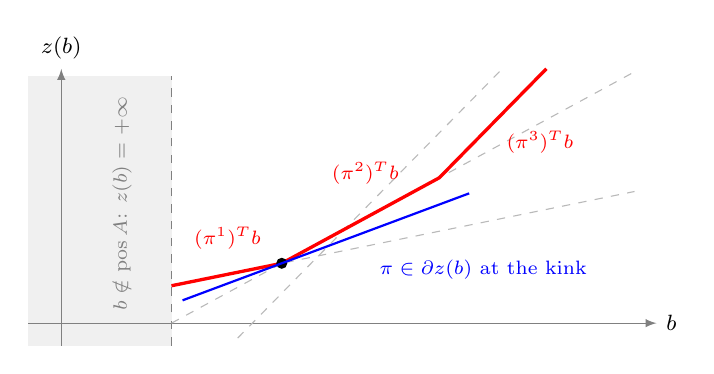
\begin{tikzpicture}[x=1.4cm,y=0.95cm,>=latex,font=\footnotesize]
  \fill[gray!12] (-0.3,-0.3) rectangle (1,3.3);
  \draw[->,gray] (-0.3,0) -- (5.4,0) node[right,black]{$b$};
  \draw[->,gray] (0,-0.3) -- (0,3.4) node[above,black]{$z(b)$};
  \draw[dashed,gray] (1,-0.3) -- (1,3.3);
  \node[gray,font=\scriptsize,align=center,rotate=90] at (0.55,1.6) {$b \notin \text{pos}\,A$: $z(b) = +\infty$};
  % the three linear pieces, extended (clipped to the plotting box)
  \begin{scope}
    \clip (-0.3,-0.3) rectangle (5.3,3.4);
    \draw[gray!55,dashed] (1,0.5) -- (5.2,1.76);
    \draw[gray!55,dashed] (1,0.0) -- (5.2,3.36);
    \draw[gray!55,dashed] (1.6,-0.2) -- (5.2,5.2);
  \end{scope}
  % envelope
  \draw[red,line width=1.2pt] (1,0.5) -- (2,0.8) -- (3.4286,1.943) -- (4.4,3.4);
  \node[red,font=\scriptsize,above left] at (1.9,0.85) {$(\pi^1)^Tb$};
  \node[red,font=\scriptsize,above left] at (3.15,1.72) {$(\pi^2)^Tb$};
  \node[red,font=\scriptsize,below right] at (3.95,2.7) {$(\pi^3)^Tb$};
  % a supporting line at the kink, with a slope strictly between the two pieces
  \fill (2,0.8) circle (2pt);
  \draw[blue,line width=0.8pt] (1.1,0.305) -- (3.7,1.735);
  \node[blue,font=\scriptsize,right] at (2.8,0.72) {$\pi \in \partial z(b)$ at the kink};
\end{tikzpicture}
\end{center}

\vspace{-2mm}

{\footnotesize One linear piece per optimal dual vertex. At a kink two bases are optimal and the subgradient is not unique --- the blue supporting line is one choice among many; elsewhere the slope is the unique optimal dual solution $\pi^*$. This is the function that recourse models differentiate, with $b = h(\xi) - T(\xi)x$.}

\end{frame}

\begin{frame}
\frametitle{References}

\begin{itemize}
\item
D. Bertsimas and J.N. Tsitsiklis, \emph{Introduction to Linear Optimization}, Athena Scientific, 1997 (Chapters 2--4).
\item
V. Chv\'atal, \emph{Linear Programming}, Freeman, 1983.
\item
A. Schrijver, \emph{Theory of Linear and Integer Programming}, Wiley, 1986 (Chapters 7--8, for Farkas' lemma and polyhedral theory).
\item
J.R. Birge and F. Louveaux, \emph{Introduction to Stochastic Programming}, 2nd edition, Springer, 2011 (Chapter 3, for the value function and the recourse problem).
\end{itemize}

\mbox{}

The Lagrangian, the general KKT conditions and the duality gap are covered in the companion {\red KKT background notes}.

\end{frame}

\end{document}
